\section{Sammanfattning av energiflöden: energibalanser}

De olika energiflödena är alltså från fasta energikällor, flöde genom väggarna, burspråk och tak, genom grunden, på grund av solinstrålning genom fönster samt på grund av ofrivillig ventilation. Den sista punkten, som orsakas av vind, utelämnas i ett första steg.

Från fasta energikällor fås alltid ett bidrag på totalt $\unit[10,5]{kW}$, se avsnitt \ref{sec:constsources}.

Ur figurerna i avsnitt \ref{sec:steadystatewall} får vi energiflödena per kvadratmeter genom de olika avsnitten av klimatskalet och med hjälp av areorna i tabell \ref{tbl:uvalue} fås det totala energiutflödet genom husets hela klimatskal.

Flödet genom grunden fås ur figur \ref{fig:cooling_ground} och solinstrålningen genom fönster en solig dag fås ur figur \ref{fig:effekt0415and1231}.


\begin{figure}[hpbt]
\centering
\subfloat[\label{fig:sum_aprnosun} Molnigt aprildygn]{
	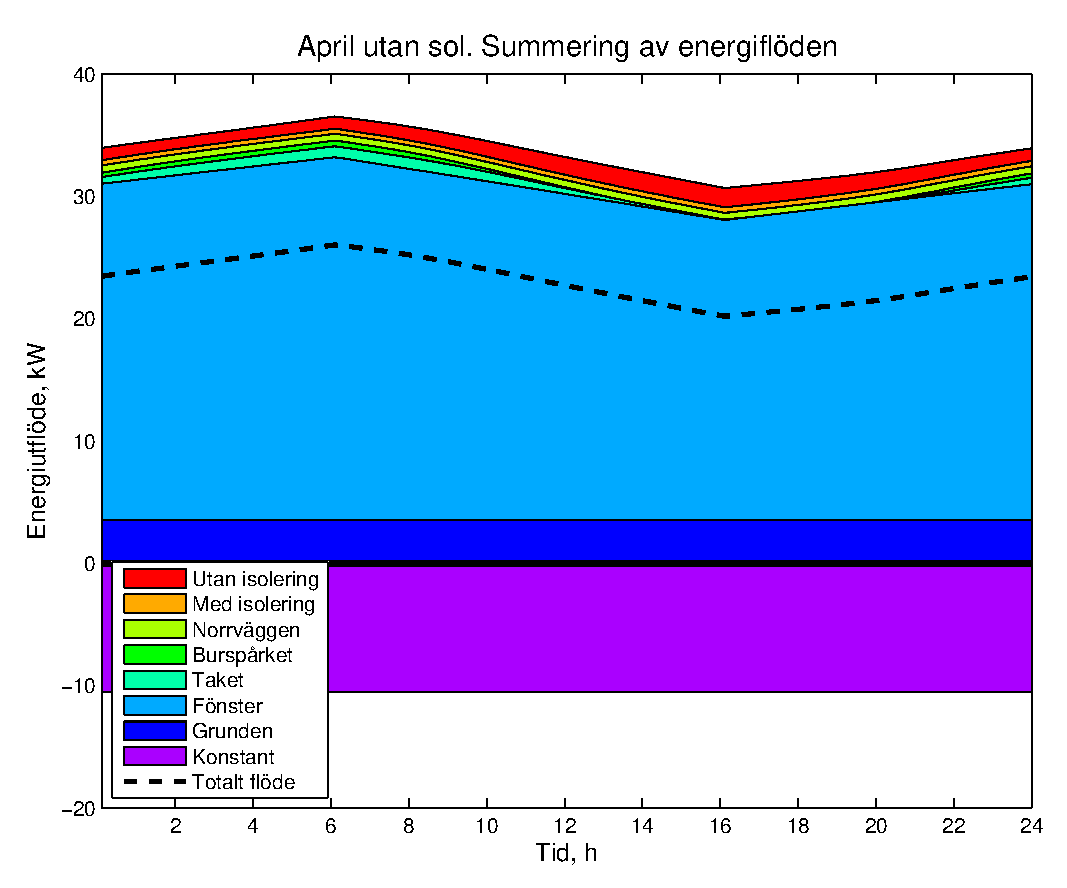
\includegraphics[width=0.45\textwidth]{images/aprnosun_sum.eps}
}
\subfloat[\label{fig:sum_aprsun} Solig aprildag]{
	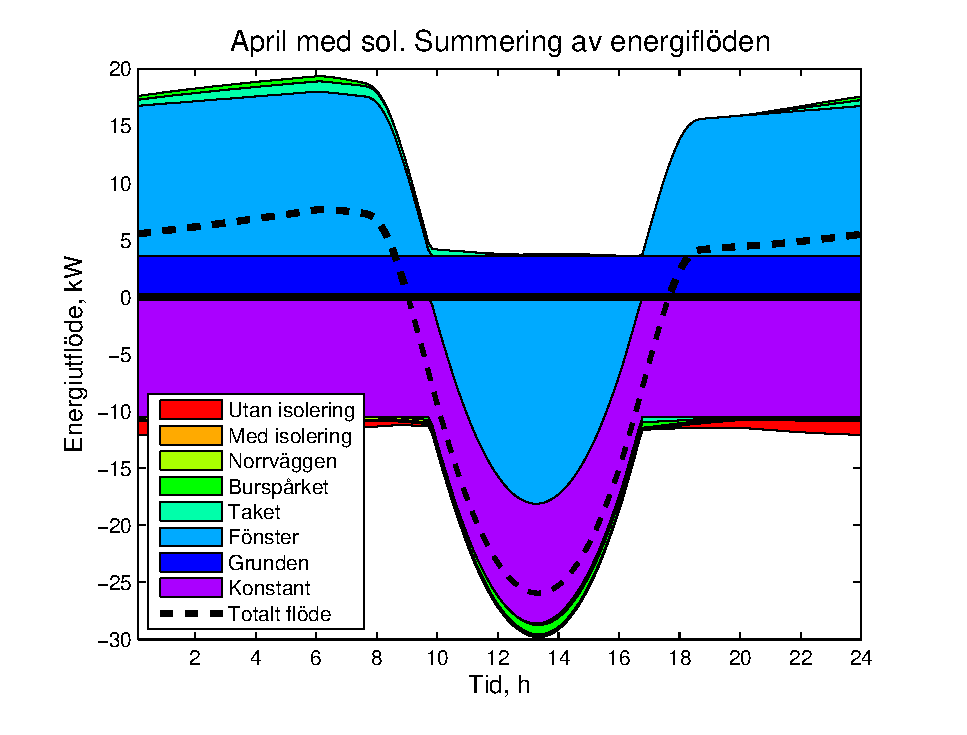
\includegraphics[width=0.45\textwidth]{images/aprsun_sum.eps}
}

\subfloat[\label{fig:sum_decnosun} Molnig decemberdag.]{
	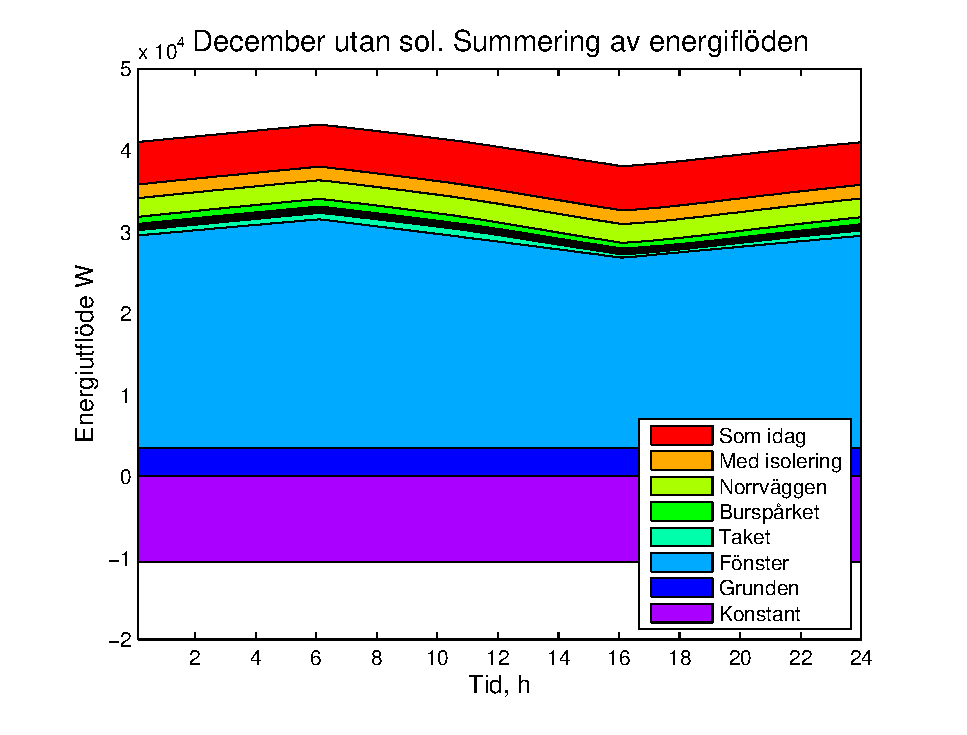
\includegraphics[width=0.45\textwidth]{images/decnosun_sum.eps}
}
\subfloat[\label{fig:sum_decsun} Solig decemberdag.]{
	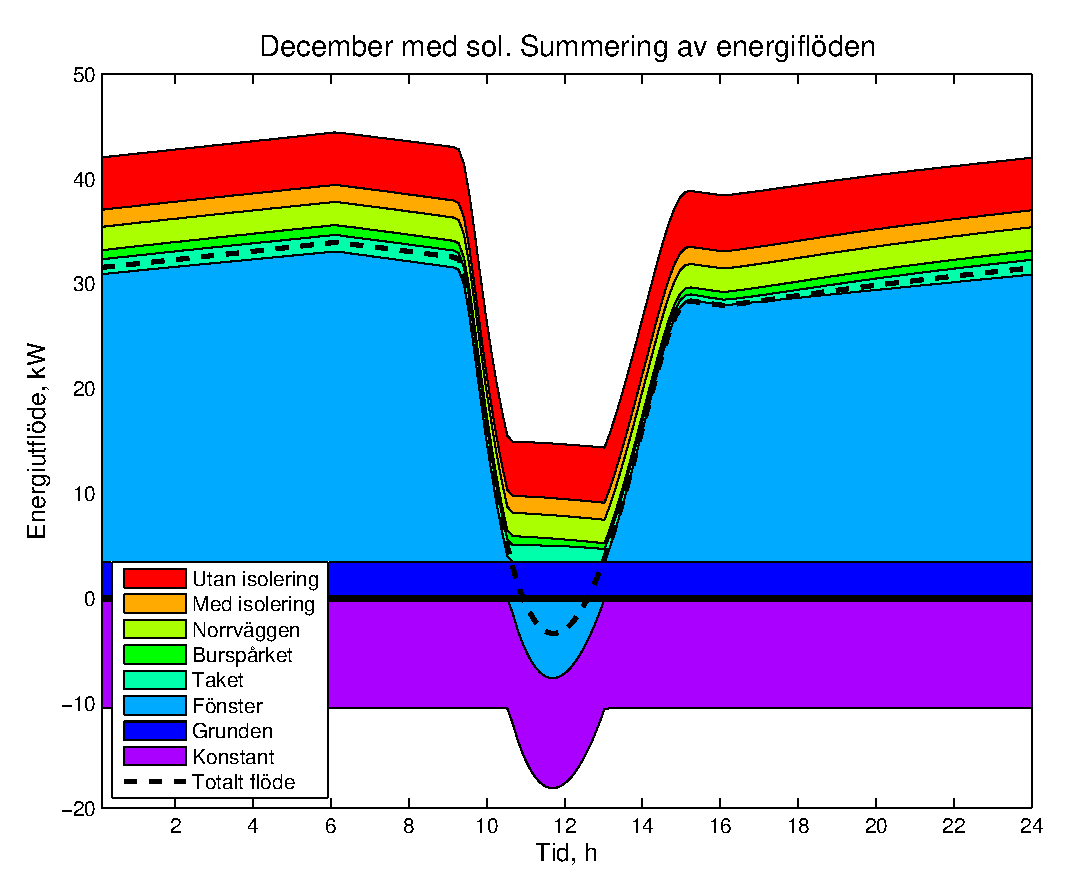
\includegraphics[width=0.45\textwidth]{images/decsun_sum.eps}
}

\caption{\label{fig:energyflow_sum} Totala energiflöden genom bygganden. Den bredare svarta linjen markerar summering av positiva och negativa energiflöden.}
\end{figure}
